\chapter{Weihrauch Reducibility and Tiling Problems}
\label{chap5}
% next resets the equation numbers to start at 1 at the start of the chapter
\setcounter{equation}{0}
\renewcommand{\theequation}{\thechapter.\arabic{equation}}

%------------------------------------------------------------------------------

\epigraph{An algorithm must be seen to be believed, and the best way to learn what an algorithm is all about is to try it.}{\textit{Donald Knuth, \\ The Art of Computer Programming, Vol. 1, 1999}}

In this chapter we will show how our constructions in the previous section can be utilised as tiling principles on represented spaces of Wang prototile sets and tilings. We present several Weihrauch reductions between these tiling problems for Wang tiles and closed choice problems.

\section{Weihrauch Reducibility}

For this section, we use \cite{Brattka2011} and \cite{Marcone2008} as our primary source material. We give a brief background overview of the theory surrounding Weihrauch reductions and their recent uses, primarily from the viewpoint of computable analysis.

\subsection{Core Concepts in Weihrauch Reducibility}

Computable analysis lends notions of computability and incomputability to computable separable metric spaces by means of notions of effective approximation. The aim is to study multi-valued functions between these spaces and to deal with their non-unique solutions. Indeed, in papers such as \cite{Weihrauch2001}, techniques from computability and reverse mathematics were combined in order to tackle a problem in computable analysis.

As Weihrauch points out in \cite{Weihrauch1995}, a core technique in computable analysis is to take notions of topological continuity and replace them with notions of computability - indeed, the explicit definition of `topologically reducible' is precisely the notion of (computably) reducible in that paper, with `computable' substituted for `continuous'. 

As such we give the following definition of reducibility for multi-valued functions (from \cite{Marcone2008}). Let $f : \subseteq X \rightrightarrows Y$ denote that $f$ is a multi-valued function with $dom(f) \subseteq X \wedge ran(f) \subseteq Y$. The idea is to take $\Pi_2$ theorems of the form $$ (\forall x \in X) \, (\exists y \in Y) \, [ (x,y) \in A ] $$ as operations $f : \subseteq X \rightrightarrows Y$ such that $$x \mapsto \{ y \in Y : (x,y) \in A \}$$ Note that the `$: \subseteq$' here indicates the (potential) partiality of our functions.

\textbf{Core Idea}: As given by \cite{Brattka2011}, the core idea for Weihrauch reducibility in relation to the choice and boundedness conditions we will study here is that, rather than defining our problems directly, we ask instead what can be understood by means of negative information. That is - if we obtain a set $X$ by negative information, say by enumeration of the complement of $X$, then how difficult is it to actually find a member of $X$? Can we define $\chi_X$ this way?

We shall put these ideas more formally:

\begin{definition}
A \emi{represented space} \textbf{X} is a pair $(X, d_X)$ where $X$ is a set and $d_X :\subseteq \omega^\omega \rightarrow \textbf{X}$ is a partial surjective function.
\end{definition}

An intuitive definition is given by Weihrauch in \cite{Weihrauch1995}:

\begin{definition}[Notations and Representations]
Using the notation for surjective partial functions above, and with $\Sigma$ denoting a finite alphabet, with $\Sigma^{<\omega}$ and $\Sigma^\omega$ denoting finite and infinite strings from $\Sigma$ respectively.
\begin{enumerate}
\item A \emi{naming system} of a set, $M$, is a surjective function $\nu : \subseteq \Sigma^{<\omega} \rightarrow M$, essentially naming every element of $M$ with finite strings.
\item A \emi{representation} is a surjective function $\delta : \subseteq \Sigma^\omega \rightarrow M$, essentially naming by infinite sequences.
\end{enumerate}
\end{definition}

Weihrauch then gives the following definition of \emph{reducibility}:
\begin{definition}
For $Y, Y^\prime \in \{ \Sigma^{<\omega}, \Sigma^\omega \}$, and for functions $\gamma : \subseteq Y \rightarrow M$ and $\gamma^\prime : \subseteq Y^\prime \rightarrow M$, we say that $ \gamma \leq \gamma^\prime $ if and only if $$ \forall y \in dom(\gamma) \, [ \gamma(y) = \gamma^\prime(f(y)) ] $$ for some computable function $f : \subseteq Y \rightarrow Y^\prime$.
\end{definition}

Likewise, $(\gamma \equiv \gamma^\prime)$ if and only if $(\gamma \leq \gamma^\prime \wedge \gamma^\prime \leq \gamma)$. However, Brattka \etal in \cite{Brattka2011} give some more general, and arguably applicable, definitions. These notions of Weihrauch reducibility will require the following notion of a realizer:

\begin{definition}
For represented spaces \textbf{X} and \textbf{Y},	
\begin{itemize}
\item For some function $f : \subseteq \textbf{X} \rightrightarrows \textbf{Y}$, a function $F:\subseteq \omega^\omega \rightarrow \omega^\omega$ is a \emi{realizer} of $f$, written $F \vdash f$, if and only if $$\forall p \in d_X^{-1}(dom(f)) \, [ d_Y(F(p)) \in f(d_X(p))]$$
\item $f$ is computable if and only if it has a computable realizer.
\item $f$ is continuous if and only if it has a continuous realizer.
\end{itemize}
\end{definition}

This is more easily summarised in the following commutative diagram:

\begin{center}
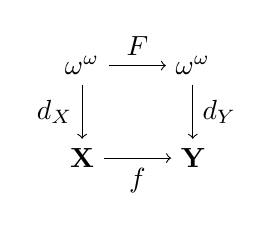
\begin{tikzpicture}[every node/.style={midway}]
  \matrix[column sep={4em,between origins}, row sep={2em}] at (0,0) {
    \node(R) {$\omega^\omega$}  ; & \node(S) {$\omega^\omega$}; \\
	\node(R/I) {$\textbf{X}$}; & \node (T) {$\textbf{Y}$};\\
  };
  \draw[<-] (R/I) -- (R) node[anchor=east]  {$d_X$};
  \draw[->] (R) -- (S) node[anchor=south] {$F$};
  \draw[->] (S) -- (T) node[anchor=west] {$d_Y$};
  \draw[->] (R/I) -- (T) node[anchor=north] {$f$};
\end{tikzpicture}
\end{center}

\begin{definition}[Weihrauch Reducibility]\label{def:Weihrauch}\index{Weihrauch reducibility}
Let $f:\subseteq \textbf{X} \rightrightarrows \textbf{Y}$ and $g :\subseteq \textbf{U} \rightrightarrows \textbf{V}$. We say that $f$ is \emph{Weihrauch reducible} to $g$, written $$ f \leq_W g$$ if there exist computable $H,K : \subseteq \omega^\omega \rightarrow \omega^\omega$, such that $$ F = K \langle id_{\omega^\omega}, GH \rangle$$ is a realizer of $f$ for every realizer $G$ of $g$.

We say that $f$ is \emi{strongly Weihrauch reducible} to $g$, written $f \leq_{sW} g$, if $$F = K(GH)$$ is a realizer for $f$.
\end{definition}

Here $\langle \cdot \rangle$ is the pairing function, as before, and $id_{\omega^\omega}$ is the identity function on Baire space. We can also say that the single-valued function $F$ is \emph{Weihrauch reducible} to $G$, also written $F \leq_W G$ if there exist single-valued computable functions $H$ and $K$ such that $$ F = K \langle id, GH \rangle $$

In \cite{Brattka2011}, these functions $H$ and $K$ are described as `functions of adaption' - $H$ being an `input adaption' and $K$ being an `output adaption'. The key idea here is to note that $H$ is the input adjustment into problems that $G$ understands, and likewise, $K$ is the transformation of the output of $G$ into an equivalent output of $F$. Thus, if $K$ does not need to know what the original input to $H$ was, represented by $id$ in Weihrauch reducibility, then the reducibility is thus defined to be stronger with respect to not needing to be `reminded' about the input that was originally fed into $H$.

Given these definitions, the following commutative diagram summarises the Weihrauch reducibility of some $f \leq_{W} g$:

\begin{center}
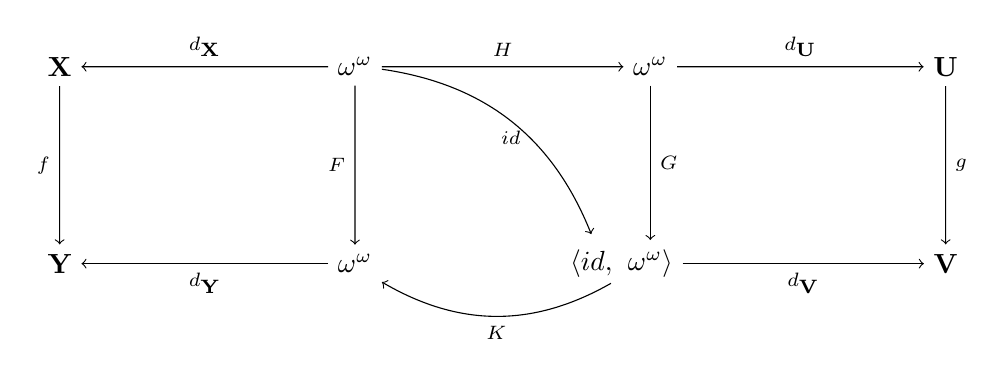
\begin{tikzpicture}[scale=2.5]
% reducing to
\node (1) at (0,1) {$\omega^\omega$};
\node (2) at (1.5,1) {$\textbf{U}$};
\node (3) at (0,0) {$\omega^\omega \rangle$};
\node (4) at (1.5,0) {$\textbf{V}$};
% reducing from
\node (A) at (-1.5,1) {$\omega^\omega$};
\node (B) at (-3,1) {$\textbf{X}$};
\node (C) at (-1.5,0) {$\omega^\omega$};
\node (D) at (-3,0) {$\textbf{Y}$};

% id
\node (id) at (-0.3,0) {$\langle id ,$};

\path[->,font=\scriptsize]
% reducing from comm. diag
(A) edge node[above]{$d_{\textbf{X}}$} (B)
(A) edge node[left]{$F$} (C)
(B) edge node[left]{$f$} (D)
(C) edge node[below]{$d_{\textbf{Y}}$} (D);

\path[->,font=\scriptsize]
% reducing to comm. diag
(1) edge node[above]{$d_{\textbf{U}}$} (2)
(1) edge node[right]{$G$} (3)
(2) edge node[right]{$g$} (4)
(3) edge node[below]{$d_\textbf{V}$} (4);

% reduction path
\path[->,font=\scriptsize]
(A) edge node[above]{$H$} (1)
(-0.2,-0.1) edge [bend left] node[below]{$K$} (C);

%id path
\draw [->,font=\scriptsize] (A) edge [bend left] node[below]{$id$} (-0.3,0.15);

\end{tikzpicture}
\end{center}

Note that the input it the arrows for $H$ and $id$ must be identical in order for the reducibility to work. Recall that for Weihrauch reducibility to be strong, we can do without this $id$ arrow and requirement, giving us the following commutative diagram which illustrates strong Weihrauch reducibility for some $f \leq_{sW} g$:

\begin{center}
\begin{tikzpicture}[scale=2.5]
% reducing to
\node (1) at (0,1) {$\omega^\omega$};
\node (2) at (1.5,1) {$\textbf{U}$};
\node (3) at (0,0) {$\omega^\omega$};
\node (4) at (1.5,0) {$\textbf{V}$};
% reducing from
\node (A) at (-1.5,1) {$\omega^\omega$};
\node (B) at (-3,1) {$\textbf{X}$};
\node (C) at (-1.5,0) {$\omega^\omega$};
\node (D) at (-3,0) {$\textbf{Y}$};

% id
%\node (id) at (-0.4,0) {$\langle id ,$};

\path[->,font=\scriptsize]
% reducing from comm. diag
(A) edge node[above]{$d_{\textbf{X}}$} (B)
(A) edge node[left]{$F$} (C)
(B) edge node[left]{$f$} (D)
(C) edge node[below]{$d_{\textbf{Y}}$} (D);

\path[->,font=\scriptsize]
% reducing to comm. diag
(1) edge node[above]{$d_{\textbf{U}}$} (2)
(1) edge node[right]{$G$} (3)
(2) edge node[right]{$g$} (4)
(3) edge node[below]{$d_\textbf{V}$} (4);

% reduction path
\path[->,font=\scriptsize]
(A) edge node[above]{$H$} (1)
(3) edge node[below]{$K$} (C);

%id path
%\draw [->,font=\scriptsize] (A) edge [bend left] node[below]{$id$} (-0.4,0.2);

\end{tikzpicture}
\end{center}


We state the following notion of \emi{realizer reducibility} from \cite{Brattka2011}:

\begin{definition}[realizer reducibility]
For $F : \subseteq \omega^\omega \rightarrow \omega^\omega$, a realizer for $f : \subseteq \textbf{X} \rightrightarrows \textbf{Y}$ ($F \vdash f$ in our notation). Let $f,g$ be multi-valued functions on represented spaces. Then $f$ is \emph{Weihrauch reducible} to $g$, $f \leq_W g$ as before, if and only if $$ \{ F : F \vdash f \} \leq_W \{ G : G \vdash g \} $$
\end{definition}

This single-valued function $F$ can be parallelized, written $\widehat{F}$, by letting $$\widehat{F} (x_0, x_1, x_2, \ldots) := F(x_0) \times F(x_1) \times F(x_2) \times \ldots$$ for some $F : \omega^\omega \rightarrow \omega^\omega$. It is shown in \cite{Brattka2011} that such parallelization is a closure operator for Weihrauch reducibility, as well as the fact that a resulting parallelized partial order forms a lattice into which the Turing and Medvedev degrees can be embedded.

Indeed, we can obtain the following proposition from \cite{Brattka2011}:
\begin{proposition}[\protect{\cite[Prop. 2.5]{Brattka2011}}]
Let $f$ and $g$ be multi-valued functions on represented spaces. Then
\begin{itemize}
\item $f \leq_W \widehat{f}$.
\item If $f \leq_W g$ then $\widehat{f} \leq_W \widehat{g}$.
\item $\widehat{f} \equiv_W \widehat{\widehat{f}}$.
\end{itemize}
\end{proposition}

Much is also made of the study of various kinds of choice in this setting, which is the subject of the next section.

\section{Weihrauch Reducibility and Choice Principles}

We now look to the Weihrauch reducibility of specific choice principles, objects that have much relevance in computable analysis. Let $C$ denote the choice principle given by 
\begin{center}
``For any set $A \subseteq \mathbb{N}$ has a characteristic function $\chi_A : \mathbb{N} \rightarrow \{0,1\}$."
\end{center}

A \emi{choice principle} or \emi{choice function} is given by this definition, and a significant amount of study is given as to the Weihrauch degrees of these functions, \eg in \cite{BrattkaPauly2010} and \cite{Brattka2011}. We shall state some of these results presently.

\begin{definition}[Compact Choice]\index{compact choice}
Let $X$ be a computable metric space, and $\mathcal{K}(X)$ be the set of compact subsets of $X$. The multivalued operation $$ CC_{\mathcal{K}(X)} : \subseteq \mathcal{K}(X) \rightrightarrows X, A \mapsto A $$ with $$dom(CC_{\mathcal{K}(X)}) := \{ A \subseteq X : A \neq \emptyset \text{ compact} \} $$ is called the \emph{compact choice} of $X$.
\end{definition}

Note, in this definition we have the inclusion of the notation ``$A \mapsto A$'', which might give the incorrect impression that we are simply mapping members in $A$ to members in $A$, but our aim is in fact rather to convey that we are mapping a given closed set $A$ to the set of its members in a multi-valued way. Our $\mathcal{K}(X)$ denotes the set of compact subsets of $X$, which are represented by enumerations of finite rational open covers which are not necessarily minimal.

\begin{definition}[Omniscience Principles]
We introduce the following principles: 
\begin{itemize}
\item Limited Principle of Omniscience (LPO) - For any sequence $\sigma \in \omega^\omega$ there exists $n \in \omega$ such that $\sigma(n) = 0 \text{ or } \sigma(n) \neq 0$ for all $n \in \omega$.
\item Lesser Limited Principle of Omniscience (LLPO) - For any sequence $\sigma \in \omega^\omega$ such that $\sigma(k) \neq 0$ for at most one $k \in \omega$, it follows that 
\begin{itemize}
\item $\sigma(2n) = 0$ for all $n \in \omega$, or 
\item $\sigma(2n+1) = 0$ for all $n \in \omega$.
\end{itemize}
\end{itemize}
\end{definition}

These notions may seem unusual, but their motivation is firmly rooted in constructive mathematics - LPO and LLPO translate the usually `forbidden' principle of excluded middle and de Morgan's laws, respectively. Though intuitionistic reasoning rejects such ideas, their representations as LPO/LLPO have realizers that correspond to discontinuous operations of varying degree of discontinuity - see \cite{Brattka2011} for details on how these and other principles, such as Markov's Principle, become somewhat unproblematic owing to their continuous, and thereby computable, realizers in this setting.

To illustrate how such a notion of choice is handled in the literature, we state the following theorem, for which the proof can be found in \cite{Brattka2011}:

\begin{theorem}[\protect{\cite[Thm. 2.10]{Brattka2011}}]\label{thm:compmetspaceLLPO}
Let $X$ be a computable metric space. Then $CC_{\mathcal{K}(X)} \leq_W \widehat{LLPO}$. If there is a computable embedding $\iota : 2^\omega \hookrightarrow X$, then $CC_{\mathcal{K}(X)} \equiv_W \widehat{LLPO}$.
\end{theorem}

We omit the proof of this, but it can be found in \cite{Brattka2011}. The following definitions are taken from \cite{Brattka2009}.

\begin{definition}[Weakly Computable]\index{weakly computable}
A function $F : \subseteq X \rightrightarrows Y$ on represented spaces $X$ and $Y$ is called \emph{weakly computable} if $F \leq_W \widehat{LLPO}$. Similarly, we also call functions like $F$ \emph{weakly continuous} given $F \leq_W \widehat{LLPO}$ holds with respect to some oracle.
\end{definition}

Based off the previous theorem \ref{thm:compmetspaceLLPO} and definition we can get the following corollary:

\begin{corollary}[\protect{\cite[Cor. 2.11]{Brattka2011}}]
Let $X$ be a represented space and let $Y$ be a computable metric space. Any weakly computable single-valued operation $F :\subseteq X \rightarrow Y$ is computable.
\end{corollary}

For our tiling problem equivalences, we will need the following definition, taken from \cite{Brattka2012} and \cite{BrattkaPauly2010}:

\begin{definition}[Closed Choice]\index{closed choice}\label{def:ClosedChoice}
Let $(\textbf{X}, d_X)$ be a represented space. Then the \emi{closed choice} operation of this space is defined by \[ C_\textbf{X} : \subseteq \mathcal{A}(\textbf{X}) \rightrightarrows \textbf{X}, A \mapsto A \] where $\mathcal{A}(\textbf{X})$ are the closed subsets of \textbf{X}, and our choice function takes some non-empty closed subset $A \in \mathcal{A}(\textbf{X})$ and outputs some point $x \in A$. We therefore have $dom(C_X) := \{ A \in \mathcal{A}(X) : A \neq \emptyset\}$
\end{definition}

We will be specifically interested in closed choice for Baire space - as this is where the trees we have been considering so far are found. \cite{Brattka2011} demonstrates how this is, in a sense, the `hardest' kind of choice, by the following definitions and theorem below. 

\begin{definition}
We define the following choice maps as follows:
\begin{enumerate}
%\item \textbf{Co-finite choice} - $$C_F : \subseteq \mathcal{A}(\omega) \rightrightarrows \omega,dom(C_F) = \{ A \subset \omega : \text{ co-finite}\} $$
\item \textbf{Discrete choice} - $$C_{\omega} : \subseteq \mathcal{A}(\omega) \rightrightarrows \omega,dom(C_{\omega}) = \{ A \subset \omega :  A \neq \emptyset\} $$
\item \textbf{Interval choice} -  $$C_I : \subseteq \mathcal{A}([0,1]) \rightrightarrows [0,1],dom(C_I) = \{ [a,b]:  0 \leq a \leq b \leq 1\} $$
\item \textbf{Proper interval choice} - $$C_I^- : \subseteq \mathcal{A}([0,1]) \rightrightarrows [0,1] ,dom(C_I^-) = \{ [a,b]: 0 \leq a \leq b \leq 1 \} $$ 
\item \textbf{Compact choice} -  $$C_K : \subseteq \mathcal{A}([0,1]) \rightrightarrows [0,1],dom(C_K) = \{ K \subseteq [0,1] : K \neq \emptyset, K \text{ compact} \} $$
\end{enumerate}

However, Brattka and Gherardi also present choice principles as boundedness principles instead of principles of choice over intervals. The intuition here stems from a similar question asked in \cite{BrattkaPauly2010}:
\begin{center}
``Given information about what does not constitute a solution, find a solution."
\end{center}
\begin{flushright}
\emph{-- Brattka, Brecht, Pauly in \cite{BrattkaPauly2010}}
\end{flushright}

So, by seeing choice principles as boundedness principles, we shift our view to the defined negative information about the represented set $A$, which is then given explicitly in the form of a finite number of bounds. It turns out that this is very useful in reducing problems in analysis - they often turn out to have a `boundedness representation'.

We find that the boundedness principle analogues of the above choice principles, given in \cite{Brattka2011}, are as follows:

\begin{enumerate}
%\item $B_F : \mathbb{R}_< \rightrightarrows \mathbb{R}, x \mapsto [x,\infty)$
\item $B : \mathbb{R}_< \rightarrow \mathbb{R}, x \mapsto x$
\item $B_I : \mathbb{R}_< \times \mathbb{R}_> \rightrightarrows \mathbb{R}, (x,y) \mapsto [x,y], dom(B_I) = \{ (x,y):x \leq y\}$
\item $B_I^- : \mathbb{R}_< \times \mathbb{R}_> \rightrightarrows \mathbb{R}, (x,y) \mapsto [x,y], dom(B_I^-) = \{ (x,y) : x < y \}$
\item $B_I^+ : \mathbb{R}_< \times \overline{\mathbb{R}_>} \rightrightarrows \mathbb{R}, (x,y) \mapsto [x,y], dom(B_I^+) = \{ (x,y) : x \leq y \}$
\end{enumerate}

Where $\mathbb{R}, \mathbb{R}_<, \mathbb{R}_>$ are equipped with ordinary Cauchy representations $\rho$ of the real numbers, the left $\rho_<$, and right $\rho_>$ respectively.

\end{definition}

These various notions of choice illustrate the degree of detail we can command in this theory. Brattka \etal in \cite{Brattka2011} illustrate the relationships between these choice operators in the following theorem. They denote these \emi{choice chains}, indicating the relationships between choice principles, boundedness principles, and our omniscience principles.

\begin{theorem}[\protect{\cite[Thm. 3.10]{Brattka2011}}][Choice Chains]
It is obtained in \cite{Brattka2011} that:
\begin{enumerate}
\item $LLPO \leq_W C_I^- \leq_W C_I \leq_W C_K \equiv_W \widehat{LLPO} \leq_W C_A$
\item $LPO \leq_W C_\omega \leq_W B_I^+ \leq_W C_A \leq_W C \equiv_W \widehat{LPO}$
\item $LLPO \leq_W LPO$, $C_I^- \leq_W C_\omega$, $C_I \leq_W B_I^+$
\end{enumerate}
\end{theorem}

As a finale, Brattka proves the following theorem:

\begin{proposition}[\protect{\cite[Prop. 3.7]{Brattka2011}}]
$$ B \equiv_W C \equiv_W \widehat{LPO} $$
\end{proposition}

This is somewhat surprising when read out loud - all of our boundedness principles are Weihrauch equivalent to all of our (closed) choice principles, both of which are equivalent to the Limited Principle of Omniscience. This result and the background theory and definitions in Weihrauch reducibility provide the backdrop for our result we present in the next subsection.

\section{Weihrauch Reducibility and Tiling Problems}

We will look specifically at Closed Choice on Baire Space, denoted $C_{\omega^{\omega}}$, defined above.

We require a proper intuition for $C_{\omega^\omega}$ - namely that any realizer for this principle in Baire space takes a tree $T \subset \omega^{< \omega}$ as input, and returns a path through it, in keeping with our definitions above.

\begin{definition}
Let the following notations be given:
\begin{itemize}
\item Let $\mathbb{W}$ denote the set of all possible Wang tiles, represented as 4-tuples.
\item Let $\mathscr{T}_{\mathbb{W}}$ denote the class of all possible tilings of all possible Wang tiles.
\end{itemize}
\end{definition}

In the spirit of our previous definitions, we define the following class.

\begin{definition}\label{def:ChooseTiling}\index{$ChooseTiling$}
Let $ChooseTiling$ or $CT$ be a multivalued operator such that $$ CT : \subseteq \mathcal{P}(\mathbb{W}) \rightrightarrows \mathscr{T}_{\mathbb{W}}, S \mapsto \mathcal{T}_S$$
where $S$ is a set of prototiles, and $\mathcal{T}_S$ is an $S$-tiling. $ChooseTiling$ as an operator/principle takes some subset of all possible Wang prototiles $S \subset \mathbb{W}$ and returns a total planar $S$-tiling $\mathcal{T}_S$, as a tiling function $f: \mathbb{Z}^2 \rightarrow S$.
\end{definition}

Note that we do not use definition of $TILE$ from \ref{def:TILE} in this definition, as we defined $TILE$ to be a set of indices for Turing Machines. However, our realizer for $CT$ will not be computable.

Intuitively this operator takes some set of prototiles and returns a total planar tiling. Thus, a realizer for $CT$ is a function $$F :\subseteq \omega^\omega \rightarrow \omega^\omega$$ which takes some set of prototiles $S$, and outputs some infinite sequence corresponding to a total planar $S$-tiling given by the tiling function $f: \mathbb{Z}^2 \rightarrow S$

We present the following result:

\begin{theorem}[C. 2019]\label{thm:CT-SW-ClosedC}
$$ CT \equiv_{sW} C_{\omega^{\omega}} $$
\end{theorem}

\begin{proof}
As per the definition of strong Weihrauch reducibility, we require to show the following reductions hold in order to get that $CT$ and $C_{\omega^\omega}$ are strong Weihrauch equivalent:
\begin{align*}
(CT \leq_{sW} C_{\omega^{\omega}}) \, \wedge \, & (C_{\omega^{\omega}} \leq_{sW} CT) \\
\end{align*}

Denote realizers $C \vdash C_{\omega^\omega}$ and $T \vdash CT$, we thus require computable $H,K :\subseteq \omega^\omega \rightarrow \omega^\omega$ such that $$ C = K(TH)$$ as well as computable $I,J :\subseteq \omega^\omega \rightarrow \omega^\omega$ such that $$ T = J(CI)$$ which we can represent with the following commutative diagram:

\begin{center}
\begin{tikzpicture}[scale=2.5]
% reducing to
\node (1) at (0,1) {$\omega^\omega$};
\node (2) at (1.5,1) {$\mathbb{W}$};
\node (3) at (0,0) {$\omega^\omega$};
\node (4) at (1.5,0) {$\mathscr{T}_{\mathbb{W}}$};
% reducing from
\node (A) at (-1.5,1) {$\omega^\omega$};
\node (B) at (-3,1) {$\mathcal{A}(X)$};
\node (C) at (-1.5,0) {$\omega^\omega$};
\node (D) at (-3,0) {$X$};

% id
%\node (id) at (-0.4,0) {$\langle id ,$};

\path[->,font=\scriptsize]
% reducing from comm. diag
(A) edge node[above]{$d_{\mathcal{A}(X)}$} (B)
(A) edge node[left]{$C$} (C)
(B) edge node[left]{$C_{\omega^\omega}$} (D)
(C) edge node[below]{$d_{X}$} (D);

\path[->,font=\scriptsize]
% reducing to comm. diag
(1) edge node[above]{$d_{\mathbb{W}}$} (2)
(1) edge node[right]{$T$} (3)
(2) edge node[right]{$CT$} (4)
(3) edge node[below]{$d_{\mathscr{T}_{\mathbb{W}}}$} (4);

% reduction path
\path[->,font=\scriptsize]
(A) edge [bend left] node[above]{$H$} (1)
(3) edge [bend left] node[below]{$K$} (C)
(1) edge [bend left] node[above]{$I$} (A)
(C) edge [bend left] node[below]{$J$} (3);

%id path
%\draw [->,font=\scriptsize] (A) edge [bend left] node[below]{$id$} (-0.4,0.2);

\end{tikzpicture}
\end{center}

We will utilise our constructions in the proof of \ref{thm:TILE-ILL}, and notice that in that construction of tilings from trees, all the parts of our construction used in the proof are computable. This important detail will inform much of the proof of this theorem. 

Note that underlying actions of $C$ and $T$: 
\begin{itemize}
\item $C$ takes some closed subset of Baire space, a tree, and finds some infinite path through it, and returns this as its output.
\item $T$ takes some finite or infinite set of prototiles $S$ and finds some infinite sequence of tiles that corresponds to a total tiling of the plane using tiles from $S$ respecting all edge meet conditions.
\end{itemize}

We will first show that there are computable $I,J : \subseteq \omega^\omega \rightarrow \omega^\omega$ such that $T = J(CI)$ in order to prove $CT \leq_{sW} C_{\omega^\omega}$. We first notice that $T$ is a function that takes a set of prototiles and produces and infinite sequence corresponding to some infinite planer tiling. Thus, $I$ will encode information about the possible $S$-tilings in a way that we can ask $C$ to process this and give us an answer that $J$ will translate back into some tiling.

Given some prototile set $S$ as input to $T$, our computable $I$ will construct the tree of possible tilings as we saw constructed in the proof of Wang's Extension Theorem, theorem \ref{thm:WangExtension} in this thesis. Specifically, $I$ will code uniquely each tile in $S$, and then proceed to code each successively larger sequence of possible tiles in square rings of tiles, joining them into the tiling tree $T_S$ based on the required edge-match criteria. With this done, we have a full tree of valid tilings given by successively larger rings that properly extend the previous finite square patch of tiles. This encoded tiling tree $T_S$ is a subset of Baire space, and so it is this tiling tree that we supply to $C$.

Given trees are closed subsets of Baire space, this is a problem that $C$ will be able to provide an answer for. Thus for our tiling tree $T_S$, $C(T_S) = p$, with $p$ some infinite path through $T_S$. This path will represent a planar tiling, by the construction of $T_S$ by $I$.

We can take the infinite path $p$ through our tiling tree generated by $I$ and then decode this as a tiling by assigning all of the tiles for initial segment of $p$ by decoding the specific arrangement of tiles coded by $I$ into the tiling tree for our $S$. Given we computably generated $T_S$, we can match up each successive initial segment of $p$ by decoding each of the encoded tiles in $p$ without knowledge of the input to $I$, with the tiles that should be placed around the previous patch of tiles being coded in each successive segment of $p$. This is our computable function $J$ that will complete our reduction, and is essentially a computable inverse of the operation of $I$, taking a coded sequence corresponding to edge-matched finite patches of $S$-tilings and recovering a planar $S$-tiling from this.

With this now done, we have successfully shown that $T$ can be computed by means of translation of tree sets into input for $C$ by $I$, and the output of $C$ can then be reinterpreted by $J$, such that we have satisfied the requirement and shown that $T = J(CI)$ is a realizer for $CT$.

Next we prove $C_{\omega^\omega} \leq_{sW} CT$, by finding computable $H,K : \subseteq \omega^\omega \rightarrow \omega^\omega $ such that $C = K(TH)$. By our intuition above we require a computable function $H$ to convert some tree into sets of prototiles, which will then allow our realizer $T$ to construct a total planar tiling, and return this to us as output. We then require a computable $K$ to take this tiling and recover from it an infinite path, which will then be returned as one of the possible paths from our original tree.

We take the two constructions in our proof of theorem \ref{thm:TILE-ILL} to be the computable functions that we need. We will explicitly show which parts relate to this reduction for this part of the proof. 

First, note that for a given tree, converting each path into the library $\mathcal{S}$ is a computable task. Although in the previous proof, we require a path to then choose the $S_e \subset \mathcal{S}$ for our original tiling, here we can pass this prototile set to our realizer $T$ and it will give us a sequence corresponding to a tiling of the plane. Explicitly, we construct this library as follows from the proof of theorem \ref{thm:TILE-ILL}:

\begin{itemize}
\item Fix a root tile with the tuple $\langle M^L_0, \lambda^U, M^R_0, \lambda^D \rangle$ and put this tile into $\mathcal{S}$.
\item For all the $c^j_i$ and $M_i$ colour the mid-row tiles.
\item For all $c^j_i$ colour all of the quadrant tiles, and put these into $\mathcal{S}$.
\item For each point (a string) $p$ in our input tree we add column tiles for each initial segment $\sigma$ and $\sigma^\frown n$ in $p$ - note, we still take two copies of each and construct two tiles for each successive symbol in each path, as one is required to go up and the other in the mirror position downwards.
\end{itemize}

With our full library $\mathcal{S}$ constructed, we now have an infinite set of prototiles which we can pass as the input to our realizer $T$. The output from this will be a planar tiling about which we already know the useful properties, namely that from this we can recover the path coded in each of the $\mathcal{S}$-tilings.

We can extract the path from an $\mathcal{S}$-tiling in the following manner. Our following computable method will be the same as the method to extract the path $p$ from our $S_e$-tiling in the proof of theorem \ref{thm:TILE-ILL}:
\begin{enumerate}
\item If we choose the root tile, read upwards along the column of tiles, from which we can recover a path $p$.
\item If we choose a mid-row tile, then we follow the descending chain of $M_i$ colours to the root tile, and then go to step 1.
\item If we choose a quadrant tile, then for our given $i \in \omega$ from our chosen tile:
\begin{itemize}
\item If $c^1_i$ or $c^2_i$ then follow all the tiles down to the mid-row tiles, and go to step 2.
\item If $c^3_i$ or $c^4_i$ then follow all the tiles up to the mid-row tiles, and go to step 2.
\end{itemize}
\end{enumerate}

Thus we have computable functions $H$, that creates from a tree a valid input for $T$, and a computable $K$, that takes the output from $T$ and extracts an infinite path $p$ for our original tree. This is satisfying the same function as the realizer $C$, thus $C = K(TH)$ is satisfied and is a realizer for $C_{\omega^\omega}$, completing our theorem.

\end{proof}

\section{Weihrauch Reductions for Weak Planar Tilings}

We can also prove a similar result for the following tiling principle, based around the definition for $WTILE$ we originally gave in definition \ref{def:WTILE}. 

\subsection{Weihrauch Equivalence for $CWPT$}

We first need the following definition of a `wild card':
\begin{definition}
Let $*$ denote the \emi{wild card} that satisfies the edge meet conditions of any Wang prototile in $\mathbb{W}$ in a tiling function $f : \mathbb{Z}^2 \rightarrow S \cup \{ * \}$, for a given set of prototiles $S \subset \mathbb{W}$.
\end{definition}

The wild card tile is intended to give us a way of handling the `blank', or `no tile', possibility that we first encountered in our definition of $WTILE$. Thus, an infinite region that is not tiled will be mapped by infinitely many wild cards. We can now continue on and define non-total tilings of the plane by adding this wild card to our prototile sets.

\begin{definition}\label{ref:CWPT}\index{$ChooseWeakPatchTiling$}
Let $ChooseWeakPatchTiling$, shortened to $CWPT$, be such that $$ CWPT :\subseteq \mathcal{P}(\mathbb{W}) \rightrightarrows \mathscr{T}_{\mathbb{W}}, S \mapsto \mathcal{T}_S $$ where $S$ is a set of prototiles, and $\mathcal{T}_S$ is an $S$-tiling. Similar to $CT$ defined in \ref{def:ChooseTiling}, $ChooseWeakPatchTiling$, is an operator/principle that takes some subset of all possible Wang prototiles $S \subset \mathbb{W}$ such that $S$-tilings returns a connected planar, but not necessarily total, $S$-tiling $\mathcal{T}_S$ given by $$f: \mathbb{Z}^2 \rightarrow S \cup \{ * \}$$ where $*$ is the `tiling wild card' defined above. $CWPT$ also returns an infinite connected region $R \subseteq \mathbb{Z}^2$ which is covered by this infinite connected patch of tiles.
\end{definition}

The following result can now be demonstrated:

\begin{theorem}[C. 2019]\label{thm:CWPT-SW-ClosedC}
$$ C_{\omega^\omega} \equiv_{sW} CWPT $$
\end{theorem}

\begin{proof}
We first reiterate that we are explicitly after two reductions to obtain our equivalence, explicitly:
\begin{align*}
(C_{\omega^\omega} \leq_{sW} CWPT ) \wedge ( CWPT \leq_{sW} C_{\omega^\omega} )
\end{align*}

Let our realizers be $C \vdash C_{\omega^\omega}$ and $W \vdash CWPT$, with $C,T : \subseteq \omega^\omega \rightarrow \omega^\omega$. As before, we want computable $H,K,I,J : \subseteq \omega^\omega \rightarrow \omega^\omega$ such that the following diagram commutes:

\begin{center}
\begin{tikzpicture}[scale=2.5]
% reducing to
\node (1) at (0,1) {$\omega^\omega$};
\node (2) at (1.5,1) {$\mathbb{W}$};
\node (3) at (0,0) {$\omega^\omega$};
\node (4) at (1.5,0) {$\mathscr{T}_{\mathbb{W}}$};
% reducing from
\node (A) at (-1.5,1) {$\omega^\omega$};
\node (B) at (-3,1) {$\mathcal{A}(X)$};
\node (C) at (-1.5,0) {$\omega^\omega$};
\node (D) at (-3,0) {$X$};

% id
%\node (id) at (-0.4,0) {$\langle id ,$};

\path[->,font=\scriptsize]
% reducing from comm. diag
(A) edge node[above]{$d_{\mathcal{A}(X)}$} (B)
(A) edge node[left]{$C$} (C)
(B) edge node[left]{$C_{\omega^\omega}$} (D)
(C) edge node[below]{$d_{X}$} (D);

\path[->,font=\scriptsize]
% reducing to comm. diag
(1) edge node[above]{$d_{\mathbb{W}}$} (2)
(1) edge node[right]{$W$} (3)
(2) edge node[right]{$CWPT$} (4)
(3) edge node[below]{$d_{\mathscr{T}_{\mathbb{W}}}$} (4);

% reduction path
\path[->,font=\scriptsize]
(A) edge [bend left] node[above]{$H$} (1)
(3) edge [bend left] node[below]{$K$} (C)
(1) edge [bend left] node[above]{$I$} (A)
(C) edge [bend left] node[below]{$J$} (3);

%id path
%\draw [->,font=\scriptsize] (A) edge [bend left] node[below]{$id$} (-0.4,0.2);

\end{tikzpicture}
\end{center}

We will prove the more straightforward of the two first, namely that $CWPT \leq_{sW} C_{\omega^\omega}$. To do this, we will require our two computable functions $I,J$ to be such that $$ W = J(CI) $$ This will be achieved in the same way as for the proof of theorem \ref{thm:CT-SW-ClosedC}.

We begin by using our intuition from the proof of theorem \ref{thm:SNT-WELL}, where we can think of our prototile sets as coding paths through trees. As for the proof there, we let $I$ be the function that codes the tree of all possible tilings from our given prototile set, but this time we allow for each boundary enumerated into this tree to be incomplete - as we only care that our tilings are connected, not that they are total. 

Despite this, we still arrive at a tree that is some subset of $\omega^\omega$. This follows from noticing that for a given prototile set $S$, our tiling functions $f : \mathbb{Z}^2 \rightarrow S$ can be extended in the following way $$ f: \mathbb{Z}^2 \rightarrow (S \cup \{ * \}) $$ where $*$ stands for the ``no tile here" option we have now allowed for $f$ to be a weak tiling of the plane. 

For this $f$ there exists an infinite patch $P \subseteq \mathbb{Z}^2$ such that
\begin{itemize}
\item $f$ follows the tiling rules.
\item $f$ is not $*$ on $P$.
\item $P$ is connected.
\item $|P| = \infty$.
\end{itemize}

This gives us some $\xi \in \Sigma^1_1$ such that $$\exists f \, \exists P \, (\xi(f,P))$$ is true if and only if $f$ weakly tiles the plane according to our definition of $CWPT$. By \cite[p.4]{sacks_2017} we have a $\Sigma^1_1$-normal form given which allows us to rewrite this formula as $$ \exists f \, \exists P \, \exists X (\psi(f,P,X)) $$ is true for $X$ a sequence of Skolem functions and $\psi \in \Pi^0_1$. This gives us a tree with which $C$ can find a path for. Thus, our $I$ is defined and computable.

Once $C$ returns a path, this path will correspond to an infinite sequence of tiles in the plane, and so our $J$ will take this and reconstruct our tiling from the selected paths through the generated tiling tree from $I$ that $C$ has provided a path from. Thus, the input and output adaption functions $I,J$ are both computable, and by utilising $C$ we have that $W  = J(CI)$, giving us $CWPT \leq_{sW} C_{\omega^\omega}$.

Next, we will prove that $C_{\omega^\omega} \leq_{sW} CWPT$. To begin, we will once again require that our computable $H,K$ be such that $$ C = K(WH) $$ This naturally comes about given that our definition of $CWPT$ includes not just the tiling function, but the knowledge of which region is an infinite patch of the $\mathbb{Z}^2$ lattice that is tiled by tiles from $S$.

Our computable $H$ will be given by the prototile set construction similar to that given in \ref{thm:SNT-WELL} - we take the input that is some tree $T \subseteq \omega^{< \omega}$, and then generate the tile set $S$ as follows. Fix $R$ $B$, and $P$ to be `red', `blue', and `purple' respectively - effectively making certain quadrants of Wang prototiles fixed colours. The prototiles we need to create for $S$ are:

\begin{itemize}
\item Add a unique root tile $\langle R, \lambda^U, B, P \rangle $ into $S$:
\begin{center}
\sampletile{$R$}{$\lambda^U$}{$B$}{$P$}
\end{center}
\item For each path $\sigma \in [ T ]$ add the tile: $\langle R, \sigma^\frown n, B, \sigma \rangle$:
\begin{itemize}
\item \textbf{NB}: We identify the empty string $\lambda^U$ with $\sigma(0)$
\end{itemize}
\begin{center}
\sampletile{$R$}{$\sigma^\frown n$}{$B$}{$\sigma$}
\end{center}
\end{itemize}

With this, we then give this $S$ as input to $W$, which will return two things:
\begin{enumerate}
\item A tiling function $f : \mathbb{Z}^2 \rightarrow S$.
\item A region $R \subseteq \mathbb{Z}^2$ containing an infinite patch of tiles.
\end{enumerate}

Intuitively, our tilings given by the coding above are long snakes of tiles where an infinite path is coded going up from the root tile. Given we have all this information available to $K$, we can make $K$ the computable function that first chooses the minimum point in $R$ - i.e. the point $(x,y)$ that has the lowest values for $x$ and $y$ - which is the point closest to $(0,0)$. 

With this point given, we can then follow the tiles from this point down until we reach the root tile $\langle R, \lambda^U, B, P \rangle $. This is done by fixing the $x$ co-ordinate from this point, and then subtracting one from $y$ until we find the $m$ such that $ (x,y-m) = \langle R, \lambda^U, B, P \rangle $.

With this found, we can then read each initial segment of an infinite path $\sigma \in [T]$. With this recovered, we can return this as an infinite path through the original tree $T$ that has been obtained by our realizer $W$. Thus we have satisfied $C = K(WH)$ as required. 

Finally, we note that both directions give our result, $C_{\omega^\omega} \equiv_{sW} CWPT$.
\end{proof}

\subsection{Weihrauch Reducibility for Other Weak Tiling Principles}

We will first state a neat notion of compositional product used in Weihrauch reducibility - Brattka and Pauly give the following theorem in \cite{Brattka2016}:

\begin{theorem}[\protect{\cite[Prop. 3.5 \& Thm. 4.1]{Brattka2016}}]\label{thm:supCompProd}
For every $f$ and $g$, the following supremum exists:
$$ sup\{ f_0 \circ g_0 : f_0 \leq_W f \wedge g_0 \leq_W g \} $$
\end{theorem}

As such, we will define the following compositional product:

\begin{definition}[Compositional Product]
The \emi{compositional product} of $f$ and $g$, written $f \star g$, is precisely this supremum from theorem \ref{thm:supCompProd}.
\end{definition}

The core idea in this compositional product is that we can find two sub-principles $f_0$ and $g_0$ that are each Weihrauch reducible to the principles we are interested in, and then use the composition of these new principles to achieve a Weihrauch reducibility of the two original principles composed. This enables us to sequentially apply different principles in order to obtain new Weihrauch reductions - a technique that we will now utilise.

%\begin{lemma}
%$f \star g$ is a cylinder.
%\end{lemma}
%
%\begin{proof}
%Given an input pair $(p,h) \in \omega^\omega \times \mathcal{M}(\textbf{V}, \omega^\omega \times \textbf{X})$ to $id \times (f \star g)$, we can compute some $h_p \in \mathcal{M}(\textbf{V}, \omega^\omega \times \textbf{X})$ such that $(\langle q,r \rangle, u) \in h_p(y) \if and only if q = p$ and $(r,u) \in h(y)$. As such, this implies that $id \times (f \star g) \leq_{sW} f \star g$ which satisfies our claim.
%\end{proof}

Note that the proof of theorem \ref{thm:CWPT-SW-ClosedC} requires that we provide the exact location of the infinite patch containing our infinite patch tiling is returned in addition to our tiling function. However, given we expected our weakly tiling prototile set $S$ to be non-total we knew how to `read' an $S$-tiling when given a known-infinite region $R$ which was tiled by $S$.

We now explore what happens if we change these requirements to take some prototile set $S$ that is total, and return an infinite region $R \subset \mathbb{Z}^2$ and a tiling function $f : R \rightarrow S $ - thereby reducing a total tiling to a weaker tiling of the plane.

\begin{definition}[$CIPT$]\index{$CIPT$}\label{def:CIPT}
Let $ChooseInfinitePatchTiling$, or $CIPT$ be defined similarly as before $$ CIPT : \subseteq \mathcal{P}(\mathbb{W}) \rightrightarrows \mathscr{T}_{\mathbb{W}} $$ with $CIPT$ taking a set of prototiles $S$ that gives total tilings of the plane, and returning the pair $(R,t)$, composed of an infinite connected region $R \subset \mathbb{Z}^2$ with a tiling function $t : R \rightarrow S$ such that we have an infinite $S$-tiling on $R$.
\end{definition}

We now have the machinery we need to state the following theorem:

\begin{theorem}[C. 2019]\label{thm:CC-WKLstarCIPT}
$$ C_{\omega^\omega} \leq_W C_{2^\omega} \star CIPT $$
\end{theorem}

Here, $C_{2^\omega}$ denotes the Closed Choice principle on Cantor Space which is equivalent to Weak K\"onig's Lemma (WKL) which we defined in section \ref{sec:KLemmaWKL}. As such, we can pass $C_{2^\omega}$ a finitely branching infinite tree, and it will return a path through it. Our use of this in the compositional product is due to the fact that we cannot always guarantee in a weak tiling of the plane that we can easily find our infinite path in a computable way given an input prototile set that is total.

\begin{proof}
We require two principles $f$ and $g$ such that $f \leq_W C_{2^\omega}$ and $g \leq_W CIPT$ and aligned in such a way that $f \circ g \geq_W C_{\omega^\omega}$. Let our $g$ and $f$ be defined as follows:
\begin{itemize}
\item $g$ will be the principle of taking some tree $\mathcal{T} \subseteq \omega^{< \omega}$ and returning some pair $(R,t)$ with $R \subset \mathbb{Z}^2$ an infinite connected region, tiled by $t : R \rightarrow S$, and $S$ is a prototile set with total tilings of the plane for any ill-founded tree $\mathcal{T}$.
\item $f$ will be the principle that will take a pair $(R,t)$ as above, and return an infinite sequence of tiles through the infinite connected region $R$ based on the tiling $t$.
\end{itemize}
For realizers $G \vdash g$ we will make use of the construction from the proof of theorem \ref{thm:SNT-WELL}, and in the final part of the proof, we will decode an infinite path through $\mathcal{T}$ from an infinite sequence of tiles from this construction.

Our proof will come in three main parts:
\begin{enumerate}
\item We first require computable $H,K$ such that $G = K(\langle id, TH \rangle)$ is a realizer for $g$, given $T \vdash CIPT$.
\item Next, we require computable $I,J$ such that $F = J(\langle id, WI \rangle)$ is a realizer for $f$, given $W \vdash C_{2^\omega}$
\item Finally we then require computable $X,Y$ such that $C = Y(\langle id, AX \rangle)$ as a realizer for $C_{\omega^\omega}$ given $A \vdash f \circ g$.
\end{enumerate}
With $H,K,J,I,X,Y,A : \subseteq \omega^\omega \rightarrow \omega^\omega$.

By $A = FG$ from the above, we will aim to arrive at the final form $$ C = Y(\langle id, FGX \rangle) $$ is a realizer for $C_{\omega^\omega}$. We will later prove in theorem \ref{thm:DPW-CC} that $CIPT \leq_{sW} C_{\omega^\omega}$, hence we only focus on this particular direction for our theorem.

Here follows the general plan for our proof. Recall that a realizer $C$ for $C_{\omega^\omega}$ takes some Baire space tree $\mathcal{T} \subseteq \omega^{< \omega}$ and returns a path through it. Thus, we need to align our realizers such that we take this tree $\mathcal{T}$, construct some prototile library $S$ that gives total planar tilings, and then show that if we restrict our planar $S$-tilings to some infinite region $R \subset \mathbb{Z}^2$, we can still recover an infinite path through our original $\mathcal{T}$ by means of $C_{2^\omega}$, which we recall is Weak K\"onig's Lemma. We do this last step by finding some infinite sequence of tiles through $R$, and set up the construction of our $S$ such that we can recover the path through $\mathcal{T}$ by means of a path through the spanning tree of $R$.

Intuitively we want to show that even if we remove much of the structural information of a total tiling of the plane but retain some infinite part, we can still find some reduction for $C_{\omega^\omega}$ by utilising a weaker closed choice principle to `fix' the damage we did to our original tiling.

\begin{proof}[Proof of (1)] - Let $g$ be the principle that takes some tree $\mathcal{T} \subseteq \omega^{< \omega}$ as input, and returns $(R,t)$, composed of an infinite connected region $R \subset \mathbb{Z}^2$, and a tiling function $t : R \rightarrow S$, where $S$ is the prototile set that has a total planar tiling for some path $p \in [\mathcal{T}]$ given $\mathcal{T}$ is ill-founded.

Let our $H$ be the computable function that takes as input some tree in Baire space, $\mathcal{T} \subseteq \omega^{<\omega}$ and produces a prototile set $S$ given by the construction we used in the proof of theorem \ref{thm:SNT-WELL}. The resulting prototile set gives a set with a total tiling for a path in $\mathcal{T}$, given that $\mathcal{T}$ is ill-founded.

$H$ passes this prototile set $S$ to our realizer $T \vdash CIPT$ which returns our $(R,t)$ as desired for our output. As such, our computable $K$ does nothing to this, and we have that $g \leq_W CIPT$.
\end{proof}

\begin{proof}[Proof of (2)] - For this, we want $f$ to be the principle of taking some pair $(R,t)$, comprised as above of a tiling for an infinite connected region $R \subset \mathbb{Z}^2$ given by a $t : R \rightarrow S$, and we wish to return some infinite sequence of tiles through this infinite connected tiling over $R$.

To obtain our reduction, we let our computable $I$ be the function that takes some tiling on an infinite region $R$ and computably constructs a spanning tree in the graph theoretic sense by starting at some point closest to $(0,0)$ and enumerating each tile based on the von Neumann neighbourhood of the edge meets for each successive tile that has not already been enumerated. This algorithm is generally a breadth-first search along the following lines:
\begin{enumerate}
\item Choose some tile in the $S$-tiling of $R$, and set the root node of $\mathcal{T}_R$ as the empty string $\lambda$.
\item Enumerate the tiles to the upper, lower, right, and left sides if they are available as successors in the resulting tree and have not yet been enumerated into the tree.
\item Group each of the successors by whether they are upper/lower or left/right in order to obtain binary branching.
\end{enumerate}
By the end of this process we have some $\mathcal{T}_R$, a finitely branching tree, which is bounded given the finite bound on the neighbourhood around each tile. We can pass $\mathcal{T}_R$ to a realizer $W \vdash C_{2^\omega}$. This will take our bounded branching tree and give us some infinite path through it. 

With this returned, we pass this to a computable function $J$ which takes the path returned by $W$ and decodes the infinite sequence of tiles through the tiled region $R$ that $W$ has found. $J$ can computably recover this by the fact that we can program it to decode each 4-tuple as a Wang tile in our tiling, and so obtain the full infinite sequence of tiles. $J$ finally outputs this infinite sequence of tiles through $R$.
\end{proof}

Now that we have our two subordinate principles defined and shown to be Weihrauch reducible to our desired components in our compositional product, we can now complete the proof by showing how these two principles work to give our desired reduction of $C_{\omega^\omega} \leq_W C_{2^\omega} \star CIPT$.

\begin{proof}[Proof of (3)] - The final stage of this proof will show that using a realizer $A \vdash f \circ g$ will be such that $C = Y(\langle id, AX \rangle)$ is a realizer for $C_{\omega^\omega}$ for computable $X,Y : \omega^\omega \rightarrow \omega^\omega$.

Our input adaption $X$ is a `do nothing' function, passing the input tree $\mathcal{T} \subseteq \omega^{< \omega}$ to a realizer for $G$.

$G$ returns a tiling $t : R \rightarrow S$ for an infinite region $R \subset \mathbb{Z}^2$ that contains some infinite path through $\mathcal{T}$ by the process described above. However, we cannot predict enough about the structure of the tiling of $R$, and so pass this to our realizer $F \vdash f$ that can take such a tiling on an infinite region $R$ and locate an infinite sequence of tiles through this region. Given our construction of $F$ we know that we will always locate the path by means of the bounded branching on the spanning tree across $R$ which is procured by means of a breadth-first search, and given $R$ is infinite we will get our tile sequence accordingly in this composition.

Our output adaption $Y$ works as follows: Recall that the prototile set $S$ generated inside $G$, taken from the proof of theorem \ref{thm:SNT-WELL}, has some coding of an initial segment $\sigma$ of the path $p$ we desire in every prototile, thus we can take the infinite sequence of tiles given by the realizer $F$ and computably decode each initial segment of $p$ in turn.

Our tile sequence may begin on any tile, but this will give us some initial segment $\sigma \prec p$, and although its immediate neighbours may not give us additional bits, it is certain that some tile at some point will give us some additional bit $i \in \omega$ that such that $\sigma^\frown i \prec p$. This is guaranteed by the fact that the construction of our prototile set $S$ has longer initial segments of $p$ found in any direction you care to look, so as long as $R$ is infinite and we find some infinite path through it, we will certainly recover an infinite path in $p \in [\mathcal{T}]$ by means of this process.

As such, the composition of $f \circ g$ and the corresponding composition of the various realizers and input and output adaption functions $X,Y$, we can conclude that that input is a tree $\mathcal{T}$ in Baire space, and the output is a path through this tree $\mathcal{T}$, which is precisely the function of $C_{\omega^\omega}$, completing our reduction.
\end{proof}

Given this, we have our final result by the combination of $f \circ g$ as the compositional product equivalent to $C_{\omega^\omega}$ giving our desired result $$ C_{\omega^\omega} \leq_W C_{2^\omega} \star CIPT $$
\end{proof}

It should be noted that the \textbf{AIT} and \textbf{PIT} constructions given by definition \ref{def:AITPIT} could not be utilised in this proof, at least not without significant rework. The most immediate construction was that given for the proof of \ref{thm:SNT-WELL}.

\section{General Weihrauch Reducibility for Wang Domino Problems}

Let the following definition for the general ``Domino Problem for Wang Tiles'' principle be given as follows.

\begin{definition}\label{def:DPW}\emi{Domino Problem for Wang Tiles Principle}
Let $\mathbb{W}$ denote the set of all possible Wang prototiles, and $\mathscr{T}_\mathbb{W}$ be the set of all possible tilings given by all possible Wang prototiles. Let the general principle of ``Domino Problems for Wang Prototile Sets'', $DPW$, be given by $$ DPW : \subseteq \mathcal{P}(\mathbb{W}) \rightrightarrows \mathscr{T}_\mathbb{W}, S \mapsto \mathcal{T}_S $$ where $S \subset \mathbb{W}$ and $\mathcal{T}_S$ is the class of all $S$-tilings. 

Our input for $DPW$ is some prototile set $S \subset ( \mathbb{W} \cup \{ * \} )$, and our output is a planar tiling, given as a tiling function $f : \mathbb{Z}^2 \rightarrow (S \cup \{ * \} )$ that meets our edge requirements and has some infinite connected patch.
\end{definition}

Note that we intend $DPW$ to be the universal multivalued function from any set of prototiles $S$ to any possible $S$-tiling that has an infinite connected region. Our aim is to show that any additional requirements on Wang tilings are essentially captured by the closed choice principle on Baire space.

Given this is the general principle that governs any domino problem for sets of Wang prototiles, the following reducibility will apply to any given Domino Problem as a general case of sections of the proofs in this chapter.

\begin{theorem}[C. 2019]\label{thm:DPW-CC}
$$ DPW \leq_{sW} C_{\omega^\omega} $$
\end{theorem}

This would appear to be intuitively true, given that our method for capturing all possible tilings of any Wang prototile set on a tiling tree, that this tree is always constructable. 

\begin{proof}
We first note that every tiling problem is generally of the following form
\begin{align}\label{eq:DPW-Pi12}
	\forall X \, \exists Y \, (\varphi(X) \rightarrow \psi(X,Y)) 
\end{align}
where $$X \subset ( \mathbb{W} \cup \{ * \} ) $$ is a set of Wang prototiles that also permits the wild card $*$, which we used in the proof of theorem \ref{thm:CWPT-SW-ClosedC}, and $Y$ is a set that encodes a tiling of the $\mathbb{Z}^2$ lattice, and $\varphi$ and $\psi$ are arithmetical functions such that:
\begin{itemize}
\item $\varphi(X)$ holds if $X$ is a valid set of Wang prototiles.
\item $\phi(X,Y)$ holds if $Y$ is a valid $X$-tiling.
\end{itemize}

By this formulation, we see that the formula \ref{eq:DPW-Pi12} is in $\Pi^1_2$, and we can thus obtain the following normal form for this (see \cite[p.6]{sacks_2017} for how this is done) given by: $$ \forall X \, \exists Y \, \theta(X,Y) $$ where $\theta \in \Pi^0_1$, $X$ is our prototile set as before, and $Y$ captures all Skolem functions that give our $X$-tilings.

By Lemma \ref{lemma:trees-rec-rels}, it follows that any domino problem can be defined in this way, and is thereby representable by a path $p = [T]$ for some $\Pi^0_1$ tree $T \subset \omega^{< \omega}$. 

Given $C_{\omega^{\omega}}$, by definition, takes a tree that is a subset of Baire space and returns a path, our Weihrauch reduction follows.
\end{proof}

Intuitively, this theorem shows that our tiling trees that we have made use of are always of the correct kind for $C_{\omega^\omega}$ to process and return a path that encodes a planar tiling.

\subsection{Further Weak Tiling Problems}\label{sec:FurtherWeakTilingProblems}

There are other weak tiling problems we can consider, although they are currently just outside the scope of this thesis. Take the following example, $WeakInfinitePatchTiling$:

\begin{definition}\label{def:WIPT}[$WIPT$]
Let $WeakInfinitePatchTilings$, shortened to $WIPT$, be defined similarly as before $$ WIPT : \subseteq \mathcal{P}(\mathbb{W}) \rightrightarrows \mathscr{T}_{\mathbb{W}} $$ with $WIPT$ taking a set of prototiles $S$, and returning a tiling function $f : \mathbb{Z}^2 \rightarrow S \cup \{ * \}$ that we know has an infinite patch, but not where that patch is.
\end{definition}

Because of the lack of any knowledge of the resultant tiling, we do not have enough structure to gain enough information in order to extract an infinite tree without a lot of help. An initial estimate is that we would need the following in order to have a Weihrauch reducibility: $$C_{\omega^\omega} \leq_W C_{2^\omega} \star C_\omega \star WIPT$$ where $C_{\omega^\omega}$ and $C_{2^\omega}$ are closed choice on Baire space and Cantor space respectively, as before, and $C_\omega$ is the principle that takes some function $f: \omega \rightarrow \omega$ with $ran(f) \neq \omega$ as input, and outputs some $n \notin ran(f)$.
